\section{Computational approach}

\begin{figure}
  \centering
  \ifmakeplots
    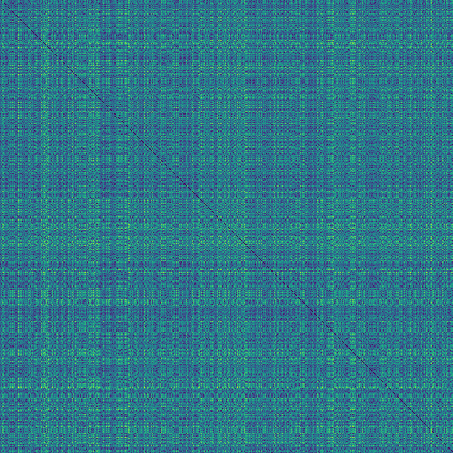
\includegraphics[width=0.4\textwidth]{figures/dist_mat_unsorted}
    \hspace{1cm}
    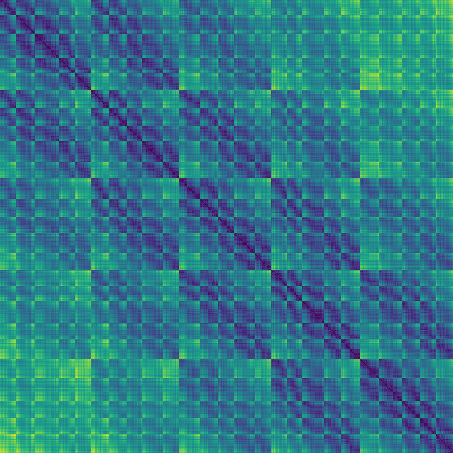
\includegraphics[width=0.4\textwidth]{figures/dist_mat_sorted}
  \fi
  \caption{\label{fig:matrix structure} the interaction matrix for $g(\vb{r}, t) = \abs{\vb{r}}^{-1}$ between points randomly distributed throughout a unit cube appears to have very little structure (left).
    While we cannot fully order the points in three dimensions, we \emph{can} permute the matrix so as to give points within the same neighborhood adjacent indices.
    Points ordered thusly produce a diagonally-dominant interaction matrix with a hierarchical Toeplitz substructure (right).
    Such structures indicate portions of the matrix have very accurate low-rank approximations that offer the possibility of significant compression.
  }
\end{figure}

\begin{figure}
  \centering
  \conditionalFigureInput{figures/aim_terminology.tex}
  \caption{\label{fig:aim terminology} Illustration of the grid structure and related terminology.
    All of the sources within a box (shown as the central shaded square) map to the same set of expansion points (shown as open circles) indexed relative to $\vb{r}_\text{box}$.
  }
\end{figure}

To effect a sub-quadratic calculation of \cref{eq:mot}, we approximate $\mathcal{F}^{(k)}$ as a sum of near- and far-field contributions.
The near-field matrix elements follow directly from \cref{eq:z elements}---sources within a prescribed distance threshold interact ``directly'' so as to avoid incurring unreasonable approximation error between adjacent basis functions.
Sources beyond this threshold, however, interact via auxiliary spatial basis functions taken to reside at the vertices of a regular Cartesian grid.
These auxiliary sources recover $\mathfrak{F}\qty{g(\vb{r}, t) \ast \vb{P}(\vb{r}, t)}$ at large distances and have two computational advantages:
\begin{inparaenum}[(i)]
  \item they compress the interaction matrix by representing sources within the same spatial region in terms of the same auxiliary set (\cref{fig:aim terminology}) and
  \item they impose a Toeplitz structure on the resulting interaction matrix that lends itself to efficient diagonalization through application of an FFT.
\end{inparaenum}
One iteration of our algorithm, then, proceeds as follows:
\begin{enumerate}
  \item At timestep $m$ project each of the $\vb{s}_\ell(\vb{r}) \mathcal{A}^\qty(m)_\ell$ onto the auxiliary sources.
    Aside from discretization/sampling criteria, the operators in \cref{eq:propagator} do not affect these projections, thus the distribution of auxiliary sources, $\vb{P}_\text{aux}(\vb{r}, t)$, mimics the distribution of $\vb{P}(\vb{r}, t)$ at large distances.
  \item Effect the convolution in \cref{eq:propagator} between auxiliary sources.
    Having imposed a regular structure on $\vb{P}_\text{aux}(\vb{r}, t)$, we may efficiently diagonalize the matrix representing this (discrete) convolution with (up to four-dimensional) blocked FFTs.
    Note that the algorithm thus far has essentially evaluated the potential, $g(\vb{r}, t) \ast \vb{P}(\vb{r}, t)$, at $t = m \, \Delta t$ at every point $\vb{u}$ in the grid.
  \item Recover the total field under the action of $\mathfrak{F}$ by projecting the potential on each $\vb{u}$ back onto the $\vb{s}_\ell(\vb{r})$.
    These projections make use of specialized projection matrices that depend on the particular derivatives contained inside $\mathfrak{F}$.
  \item Subtract the fields determined by steps 1-3 for pairs of spatial basis functions within a prescribed distance threshold and replace it with \cref{eq:z elements}.
    The auxiliary grid approximations only remain accurate at large distances, thus this step corrects large approximation errors that occur between adjacent $\vb{s}_\ell(\vb{r})$.
\end{enumerate}
Mathematically,
\begin{equation}
  \begin{aligned}
    \mathcal{F}^\qty(m - m') & \approx \mathcal{F}^\qty(m-m')_\text{direct} + \Lambda_\mathfrak{F} \mqty(\partial_t^0 \mathcal{G}^\qty(m-m') \\ \partial_t^1 \mathcal{G}^\qty(m-m') \\ \partial_t^2 \mathcal{G}^\qty(m-m') \\ \vdots) \Lambda^\dagger \\
                             & \equiv \mathcal{F}^\qty(m-m')_\text{direct} + \mathcal{F}^\qty(m-m')_\text{FFT}
    \end{aligned}
  \label{eq:f decomposition}
\end{equation}
where
\begin{subequations}
  \begin{align}
    \mathcal{F}^\qty(m-m')_{\text{direct},\ell\ell'} &= \begin{cases}
      \mathcal{F}^\qty(m-m')_{\ell\ell'}  - \mathcal{F}^\qty(m-m',\tau)_{\text{FFT},\ell\ell} & R_{\ell\ell'} \leqslant \gamma \\
      0 & \text{otherwise},
    \end{cases} \\
    \mathcal{G}^\qty(m-m')_{ab} &= \left< \vb{u}_a(\vb{r})\delta\qty\big(t - (m-m')\, \Delta t), g(\vb{r}, t) \ast \vb{u}_{b}(\vb{r})T(t) \right>
  \end{align}
  \label{eq:decomposition elements}
\end{subequations}
The $\Lambda$ matrices in \cref{eq:f decomposition} denote the (sparse) projections to and from the grid (detailed in \cref{sec:expansion matrices}), and $\vb{u}_a(\vb{r})$ indicates an auxiliary basis function on the spatial grid indexed by $a$.
Finally, $\tau_\text{max}$ and $\gamma$ serve as adjustable input parameters to control the accuracy of the simulation and $R_{\ell\ell'}$ gives the minimum distance (in integral units of the grid spacing) between the expansion regions enclosing $\vb{s}_\ell(\vb{r})$ and $\vb{s}_{\ell'}(\vb{r})$ (\cref{fig:nearfield criterion}) via
\begin{equation}
  R^\text{grid}_{\ell\ell'} = \min\!\qty{\norm{\vb{u} - \vb{u}'}_\infty \, | \, \vb{u} \in C_\ell, \, \vb{u}' \in C_{\ell'}}.
\end{equation}

\begin{figure}
  \centering
  \conditionalFigureInput{figures/nf_pair.tex}
  \caption{\label{fig:nearfield criterion}Illustration of the nearfield criterion for a third order expansion ($\gamma = 2$).
    The dashed line indicates the complete nearfield of the box associated with \textcolor{cbblue}{$\vb{r}_0$}---i.e. all boxes that have an expansion point within $\Delta s$ of the expansion around \textcolor{cbblue}{$\vb{r}_0$}.
    Consequently, all of the $\vb{s}_\ell(\vb{r})$ within the central dark blue square have a pairwise interaction with the $\vb{s}_{\ell'}(\vb{r})$ inside the dashed box.
  }
\end{figure}

\begin{figure}
  \centering
  \conditionalFigureInput{figures/nf_correction}
  \caption{\label{fig:nearfield correction}Illustration of nearfield corrections between close boxes.
    Expansions $A$ and $B$ overlap, but only box $B$ lies in the nearfield of box $C$.
    The grid-based propagation strategy only remains accurate for distant source/observer pairs.
    To avoid incurring undue error, we remove the interaction ``through the grid'' between the $BC$ pair (red line) and replace it with a more accurate ``direct'' interaction (dashed blue line).
    The $AC$ pair requires no such treatment as they have well-separated expansion regions.
  }
\end{figure}

\subsection{\label{sec:expansion matrices}Expansion matrices}

We represent the primary $\vb{s}_\ell(\vb{r})$ basis functions as a weighted sum of $\delta$-functions on the surrounding gridpoints, thus $\vb{u}_a(\vb{r}) \propto \delta(\vb{r} - \vb{r}_a)$ and
\begin{equation}
  \psi_\ell(\vb{r}) \approx \sum_{\vb{u} \in C_\ell} \Lambda_{\ell\vb{u}}^\dagger \delta(\vb{r} - \vb{u}).
  \label{eq:grid linear combination}
\end{equation}
Here, $\psi_\ell(\vb{r}) \in \qty{\vb{s}_\ell(\vb{r})\cdot \vu{x}, \vb{s}_\ell(\vb{r}) \cdot \vu{y}, \vb{s}_\ell(\vb{r}) \cdot \vu{z}}$ and $C_\ell$ denotes the collection of grid points within the expansion region of $\vb{s}_\ell(\vb{r})$ (\cref{fig:aim terminology}).
For an expansion of order\footnote{In principle, one could expand to different orders in different Cartesian directions, though this involves considerably more bookkeeping for relatively little benefit. Thus, for convenience, we take ``the expansion order'' to mean the expansion order in every direction.} $m$, this sum contains $(m + 1)^3$ terms corresponding to the $(m + 1)^3$ grid points nearest to $\vb{s}_\ell(\vb{r})$ (\cref{fig:expansion pattern}).
Consequently, the $\Lambda_{\ell \vb{u}}^\dagger$ matrices contain few nonzero elements and we have elected to use a moment-matching scheme to capture the $(m + 1)^3$ multipole moments of $\vb{s}_\ell(\vb{r})$ according to
\begin{equation}
  \sint (x - x_0)^{m_x}(y - y_0)^{m_y}(z - z_0)^{m_z} \qty[\psi_\ell(\vb{r}) - \sum_{\vb{u} \in c_\ell} \Lambda_{\ell\vb{u}}^\dagger \delta(\vb{r} - \vb{u})] \dd[3]{\vb{r}} = 0.
  \label{eq:moment matching}
\end{equation}
In this expression, $0 \leqslant m_x, m_y, m_z \leqslant m$ and $\vb{r}_0 \equiv x_0 \vu{x} + y_0 \vu{y} + z_0\vu{z}$ denotes the origin about which we compute the multipoles.
To determine the $\Lambda_{\ell \vb{u}}^\dagger$, we then solve the least-squares system
\begin{equation}
  \sum_{\vb{u} \in C_\ell} W_{\vb{m}\vb{u}}\Lambda_{\ell\vb{u}}^\dagger = Q_{\ell\vb{m}}
  \label{eq:expansion matrix system}
\end{equation}
where
\begin{subequations}
  \begin{align}
    W_{\vb{m}\vb{u}} &= (u_x - x_0)^{m_x} (u_y - y_0)^{m_y} (u_z - z_0)^{m_z} \label{eq:w matrix} \\
    Q_{\ell \vb{m}} &= \int_{} \psi_\ell(\vb{r}) (x - x_0)^{m_x} (y - y_0)^{m_y} (z - z_0)^{m_z} \dd[3]{\vb{r}} \label{eq:q vector},
  \end{align}
\end{subequations}
$\vb{u} \in C_\ell$, and $\vb{m}$ denotes the multi-index $\vb{m} = \qty{m_x, m_y, m_z}$.
With an infinite precision calculation, the choice of $\vb{r}_0 = x_0 \vu{x} + y_0 \vu{y} + z_0 \vu{z}$ merely defines an origin for the polynomial expansion system.
To minimize numerical issues, we choose $\vb{r}_0$ at the center of $\vb{s}_\ell(\vb{r})$.

As $\Lambda^\dagger$ arises purely as a function of space with no time component, differentiating \cref{eq:moment matching} with respect to $x$, $y$, or $z$ can also recover spatial derivatives occurring in $\mathfrak{F}$.
We interpret this as as differentiating the underlying polynomial that interpolates the potential between gridpoints at the location of $\vb{s}_\ell(\vb{r})$, thus the differentiation procedure removes the high-order moments in \cref{eq:q vector}.

\begin{figure}
  \centering
  \conditionalFigureInput{figures/expansion-grid}
  \caption{\label{fig:expansion pattern}Spatial expansion pattern for $\vb{s}_\ell(\vb{r}) = \vu{d}_\ell \delta(\vb{r} - \vb{r}_\ell)$ through order five.
    The numbers on the grid indicate the points added in the equivalent order expansion such that an expansion of order $m$ requires $(m + 1)^3$ grid points.
    Moreover, increasing the expansion order incorporates new points in such a way as to keep $\vb{s}_\ell(\vb{r})$ as close to the center of the expansion region as possible.
  }
\end{figure}

\subsection{Complexity}

We have largely designed this acceleration algorithm to accommodate time-domain propagators within a rotating-wave/envelope-tracking framework.
Such systems notably have decoupled length and time scales; downshifting a narrow-band signal to baseband (in time) affords very efficient temporal discretizations due to an assumed carrier signal.
No such trick works for the spatial properties, however, due to the space/time coupling in $g(\vb{r}, t)$ and need to preserve interference phenomena throughout space\footnote{Because of this, rotating-wave systems share a large number of similarities with their fully frequency-domain counterparts.}.
As such, $g(\vb{r}, t)$ can impose a high spatial frequency on fields radiating from artificially low-frequency sources.
Consequently, the both the primary and auxiliary spatial basis functions require a discretization on the order of this spatial frequency to accurately sample fields.
The calculation of \cref{eq:f decomposition}, then, remains the dominant factor in the complexity of our algorithm, though it performs significantly better than a pairwise interaction between all of the $\vb{s}_{\ell}(\vb{r})$.
Projecting sources to/from the auxiliary grid (i.e. right-multiplying by $\Lambda_\mathfrak{F}$ or $\Lambda^\dagger$) necessarily require $\mathcal{O}(N_s)$ operations per timestep as each $\vb{s}_\ell(\vb{r})$ maps to a fixed number $\vb{u}_a(\vb{r})$ auxiliary functions, independent of $N_s$.
Similarly, for uniformly-dense volume-filling geometries, a volume proportional to $\gamma^3$ contains a fixed number of $\vb{s}_\ell(\vb{r})$ independent of $N_s$, ergo the calculation of $\mathcal{F}_\text{direct}^\qty(m-m') \mathcal{A}^\qty(m')$ also requires $\mathcal{O}(N_s)$ operations.
Thus, the potential evaluation between auxiliary functions---multiplying by $\mathcal{G}^\qty(m-m')$ and its derivatives---dominates the overall complexity of the calculation.
By storing a diagonal, $\vb{k}$-space representation of these matrices (requiring storage proportional only to the number of grid points, $N_\text{grid}$, not its square), each timestep in the algorithm requires an $\mathcal{O}(N_\text{grid} \log N_\text{grid})$ forward FFT to equivalently transform the auxiliary source distribution, an $\mathcal{O}(N_\text{grid})$ elementwise product to effect the ``convolution'', and a backward $\mathcal{O}(N_\text{grid} \log N_\text{grid})$ to restore the potential in $\vb{r}$- (not $\vb{k}$-) space.
Similar Toeplitz diagonalization strategies also work in time (see~\cite[section D]{Yilmaz2004}) though this provides almost no benefit in rotating-frame systems due to the relatively small number of timesteps required for radiation to traverse the system.

Additionally, we note that transferring the spatial derivatives in $\mathfrak{F}$ onto the ``receiving'' projection matrices, $\Lambda_\mathfrak{F}$, results in a modest acceleration for tensorial propagators such as that of the electric, magnetic, or combined field integral equations,
\begin{equation}
  \mathfrak{F} = \partial_t^2 -c^2 \grad \grad \boldsymbol{\cdot}.
\end{equation}
Instead of projecting both $\vb{s}_\ell(\vb{r})$ and $\div{\vb{s}_\ell(\vb{r})}$ onto the auxiliary grid and propagating them with the relatively expensive $\mathcal{G}$ multiplication, we reconstruct all spatially-varying quantities from the potential sampled on the auxiliary grid.
(A similar method reconstructs time derivatives from the history of potential samples on the auxiliary grid, though this requires a discrete convolution with several weighted $\Lambda_\mathfrak{F}$ matrices.)
Moreover, this decomposition maintains the strong form of the integral relation in \cref{eq:propagator} and makes no assumptions of differentiability in the underlying $\vb{s}_\ell(\vb{r})$ discretization.

